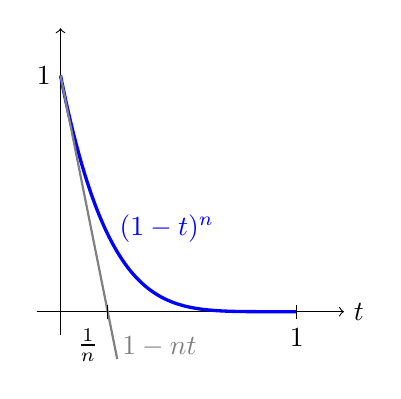
\begin{tikzpicture}[scale=3]
  \draw[->] (-0.1,0) -- (1.2,0) node[right] {$t$};
  \draw[->] (0,-0.1) -- (0,1.2);
  \draw[blue, very thick, domain=0:1, samples=80, smooth] plot (\x, {(1-\x)^5});
  \draw[gray, thick] (0,1) -- (0.24,-0.2);
  \node[left] at (0,1) {$1$};
  \draw (1,0.03) -- (1,-0.03) node[below] {$1$};
  \draw (0.2,0.03) -- (0.2,-0.03) node[below left] {$\frac1n$};
  \node[blue] at (0.45,0.35) {$(1-t)^n$};
  \node[gray, right] at (0.22,-0.15) {$1-nt$};
\end{tikzpicture}
